% chktex-file 1
% chktex-file 13
% chktex-file 26
\documentclass{article}
% chktex-file 34
% chktex-file 18
% chktex-file 1
\usepackage{amsfonts}
\usepackage[T1]{fontenc}
\usepackage{amsmath}
\usepackage{amssymb}
\usepackage{mathrsfs}
\usepackage{extarrows}
\usepackage{hyperref}
\usepackage[utf8]{inputenc}
\usepackage{graphicx}
\usepackage{mathtools}
\usepackage[a4paper, total={6in, 8in}]{geometry}
\usepackage[table]{xcolor}
\usepackage{tikz}
\usepackage{cancel}
\usepackage{steinmetz}
\usepackage{diagbox}
\usepackage{siunitx}
\usepackage{eurosym}
\usepackage{pgfplots}
\pgfplotsset{width=10cm,compat=1.9}
\usetikzlibrary{shapes,arrows}
\usepackage{listings}
\usepackage{color}
%definizione colori per blocchi di codice
\definecolor{lightgray}{rgb}{.95,.95,.95}
\definecolor{darkgray}{rgb}{.4,.4,.4}
\definecolor{purple}{rgb}{0.65, 0.12, 0.82}
\definecolor{ocherCode}{rgb}{1, 0.5, 0}
\definecolor{blueCode}{rgb}{0, 0, 0.93}
\definecolor{greenCode}{rgb}{0, 0.6, 0}

%formattazione per i blocchi di codice
\lstset{
  %Special characters
  literate={á}{{\'a}}1 {é}{{\'e}}1 {í}{{\'\i}}1 {ó}{{\'o}}1 {ú}{{\'u}}1 {Á}{{\'A}}1 {É}{{\'E}}1 {Í}{{\'I}}1 {Ó}{{\'O}}1 {Ú}{{\'U}}1 {à}{{\`a}}1 {è}{{\`e}}1 {ì}{{\`\i}}1 {ò}{{\`o}}1 {ù}{{\`u}}1 {À}{{\`A}}1 {È}{{\`E}}1 {Ì}{{\`I}}1 {Ò}{{\`O}}1 {Ù}{{\`U}}1 {ä}{{\"a}}1 {ë}{{\"e}}1 {ï}{{\"\i}}1 {ö}{{\"o}}1 {ü}{{\"u}}1 {Ä}{{\"A}}1 {Ë}{{\"E}}1 {Ï}{{\"I}}1 {Ö}{{\"O}}1 {Ü}{{\"U}}1 {â}{{\^a}}1 {ê}{{\^e}}1 {î}{{\^\i}}1 {ô}{{\^o}}1 {û}{{\^u}}1 {Â}{{\^A}}1 {Ê}{{\^E}}1 {Î}{{\^I}}1 {Ô}{{\^O}}1 {Û}{{\^U}}1 {ã}{{\~a}}1 {ẽ}{{\~e}}1 {ĩ}{{\~\i}}1 {õ}{{\~o}}1 {ũ}{{\~u}}1 {Ã}{{\~A}}1 {Ẽ}{{\~E}}1 {Ĩ}{{\~I}}1 {Õ}{{\~O}}1 {Ũ}{{\~U}}1 {œ}{{\oe}}1 {Œ}{{\OE}}1 {æ}{{\ae}}1 {Æ}{{\AE}}1 {ß}{{\ss}}1 {ű}{{\H{u}}}1 {Ű}{{\H{U}}}1 {ő}{{\H{o}}}1 {Ő}{{\H{O}}}1 {ç}{{\c c}}1 {Ç}{{\c C}}1 {ø}{{\o}}1 {Ø}{{\O}}1 {å}{{\r a}}1 {Å}{{\r A}}1 {€}{{\euro}}1 {£}{{\pounds}}1 {«}{{\guillemotleft}}1 {»}{{\guillemotright}}1 {ñ}{{\~n}}1 {Ñ}{{\~N}}1 {¿}{{?`}}1 {¡}{{!`}}1 {'"'}{\textquotesingle "\textquotesingle}3,
  %Basic design
  backgroundcolor=\color{lightgray},
  frame=l,
  % Line numbers
  xleftmargin={0.75cm},
  numbers=left,
  numberstyle=\footnotesize,
  numbersep=9pt,
  stepnumber=1,
  firstnumber=1,
  numberfirstline=true,
  % Code design
  identifierstyle=\color{black},
  keywordstyle=\color{blue}\bfseries,
  ndkeywordstyle=\color{ocherCode}\bfseries,
  stringstyle=\color{greenCode}\ttfamily,
  commentstyle=\color{darkgray}\ttfamily,
  %Code
  columns=[c]fixed,
  extendedchars=true,
  upquote=true,
  breaklines=true,
  showstringspaces=false,
  showspaces=false,
  tabsize=2,
  breaklines=true,
  showtabs=false,
  captionpos=b
}
%lingue supportate:
%ABAP
%ACSL
%Ada
%Algol
%Ant
%Assembler
%Awk
%bash
%Basic
%C#5
%C++
%C
%Caml
%Clean
%Cobol
%Comal
%csh
%Delphi
%Eiffel
%Elan
%erlang
%Euphoria
%Fortran
%GCL
%Go (golang)
%Gnuplot
%Haskell
%HTML
%IDL
%inform
%Java
%JVMIS
%ksh
%Lisp
%Logo
%Lua
%make
%Mathematica
%Matlab
%Mercury
%MetaPost
%Miranda
%Mizar
%ML
%Modelica
%Modula-2
%MuPAD
%NASTRAN
%Oberon-2
%Objective C
%OCL
%Octave
%Oz
%Pascal
%Perl
%PHP
%PL/I
%Plasm
%POV
%Prolog
%Promela
%Python
%R
%Reduce
%Rexx
%RSL
%Ruby
%S4
%SAS
%Scilab
%sh
%SHELXL
%Simula
%SQL
%tcl4
%TeX
%VBScript
%Verilog
%VHDL
%VRML
%XML
%XSLT

\newcommand{\acapo}{\\\hspace*{1cm}\\}
\newcommand{\Eaccentata}{$\grave{\text{E}}$ }
\newcommand{\vopen}{``}
\newcommand{\apexopen}{`}
\newcommand{\vclose}{''}
\newcommand{\vclosespace}{'' }
\newcommand{\indenta}{\hspace*{1cm}}
\newcommand{\define}{\underline{Def:} }

\setlength{\parindent}{0cm}

\hfuzz=100pt

\author{Flavio Colacicchi}

\title{Modellazione di dominio\\\normalsize Analisi e progettazione del software}
\date{17/03/2025}
\begin{document}
\maketitle
Un modello di dominio è un modello concettuale a oggetti che descrive le informazioni che devono essere gestite dal sistema, quindi il nome corretto dovrbebe essere \textbf{modello delle informazioni di dominio}, rappresentato con un diagramma UML visualizzando classi, associazioni e attributi concettuali del dominio del problema, ed è anche un dizionario visuale del linguaggio di dominio.\acapo
Si tratta dell'elaborato più importante dell'OOA ed è sviluppato in modo iterativo e incrementale limitato dai requisiti dell'iterazione corrente.\\
Eccone un esempio (parziale) basato sul sistema POS
\begin{center}
    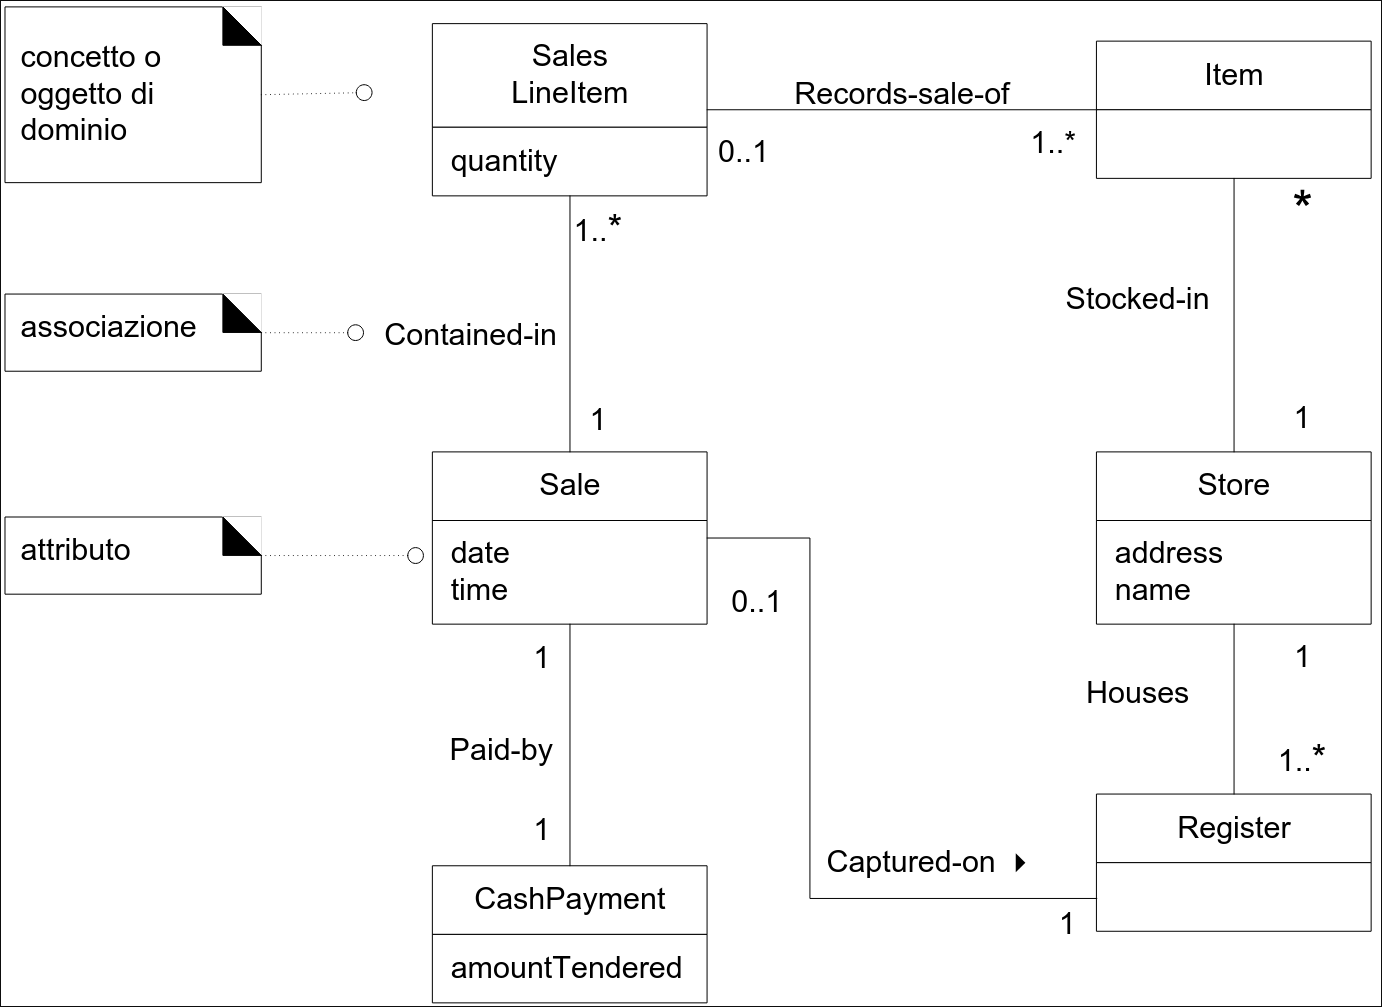
\includegraphics[width=\textwidth]{images/modello di dominio parziale pos.png}
\end{center}
Il diagramma delle classi è un termine di UML, il modello di dominio (ovvero un caso particolare del diagramma delle classi) è un termine di UP. \Eaccentata importante ricordare che questo modello è un'astrazione di oggetti reali, non diagrammi precisi di classi software, non si tratta neanche di un modello di dati, questo descrive (solo) le informazioni persistenti\footnote{Ricordato dopo l'esecuzione di ciascuna transazione/istanza di caso d'uso} di un'applicazione mentre un modello di dominio tratta tutte le informazioni che deve gestire un sistema, anche quelle transienti\footnote{Ricordato tra passi diversi dell'esecuzione di un caso d'uso} ma non quelle \vopen locale\vclosespace\footnote{Ricordato (solo) entro un singolo passo dell'esecuzione di un caso d'uso}.\acapo
Nella pratica ci sono due utilizzi del termine \vopen modello di dominio\vclose:
\begin{itemize}
    \item in UP (e in quesgto corso)\\
        descrizione concettuale degli oggetti del mondo reale di interesse
    \item Nel software\\
        Strato software composto dalle classi software usate per rappresentare oggetti del mondo reale\\
        Chiamato anche strato del dominio, composto da oggetti di dominio
\end{itemize}
Perché creare un modello di dominio?
\begin{itemize}
    \item Nell'analisi
        \begin{itemize}
            \item Per comprendere il dominio del sistema da realizzare e il suo vocabolario
            \item Per definire un linguaggio comune che abiliti la comunicazione tra le varie parti interessate
        \end{itemize}
    \item Per la progettazione\begin{itemize}
        \item Come fonte di ispirazione per progettare lo strato del dominio
        \item Per mantenere basso il salto rappresentazionale
        \item Per abilitare lo sviluppo di un sistema software facilmente comprensibile, modificabile ed evolvibile, è opportuno che una porzione del sistema rifletta il modello di dominio in modo piuttosto accurato [DDD]\footnote{Domain Driven Design}
    \end{itemize}
\end{itemize}
Il salto rappresentazionale è la distanza tra il nostro modello mentale del dominio e la rappresentazione del dominio mediante il software. Vantaggi di un salto rappresentazionale basso
\begin{itemize} 
    \item Assegnazione di responsabilità guidata dal nostro modello mentale del dominio
    \item Comprensibilità e modificabilità del progetto e del codice
\end{itemize}
\begin{center}
    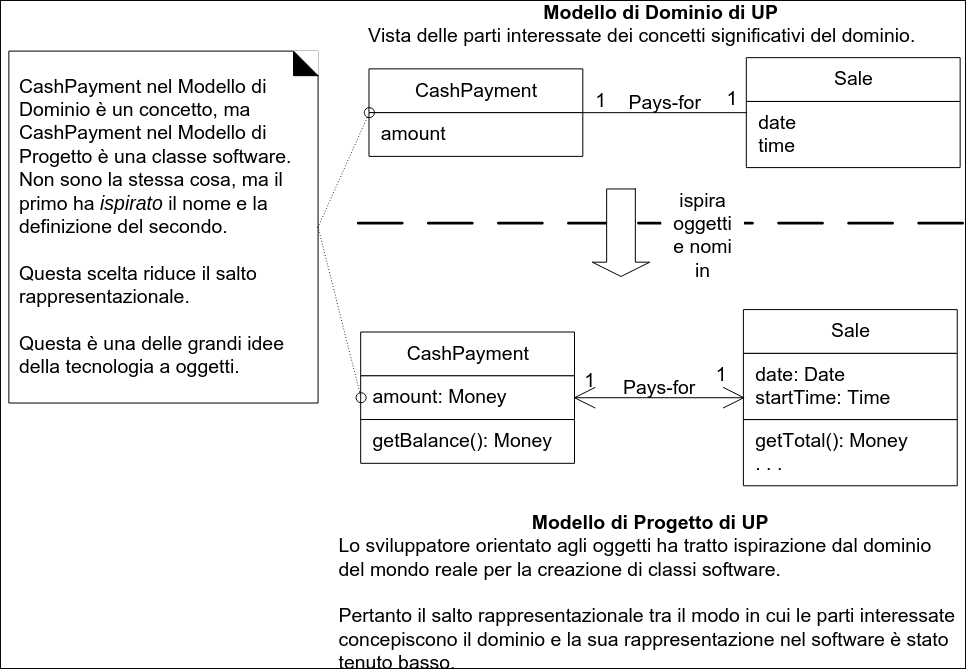
\includegraphics[width=7cm]{images/salto rappresentazionale basso.png}
\end{center}
Diagramma UML di una classe
\begin{center}
    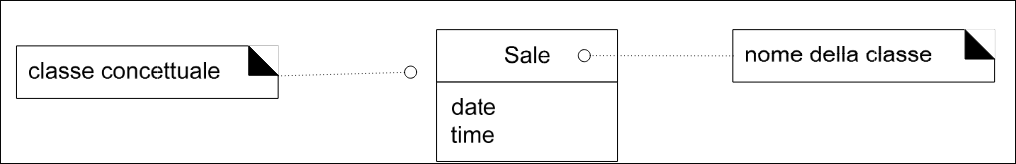
\includegraphics[width=\textwidth]{images/uml class.png}
\end{center}
In UML, possiamo usare un diagramma degli oggetti
\begin{itemize}
    \item In diagramma degli oggetti di dominio rappresenta, in modo visuale, un insieme di oggetti di esempio del mondo reale, nel contesto del dominio del problema
    \item \Eaccentata un grafo, che rappresenta oggetti, collegamenti e valor
\end{itemize}
\begin{center}
    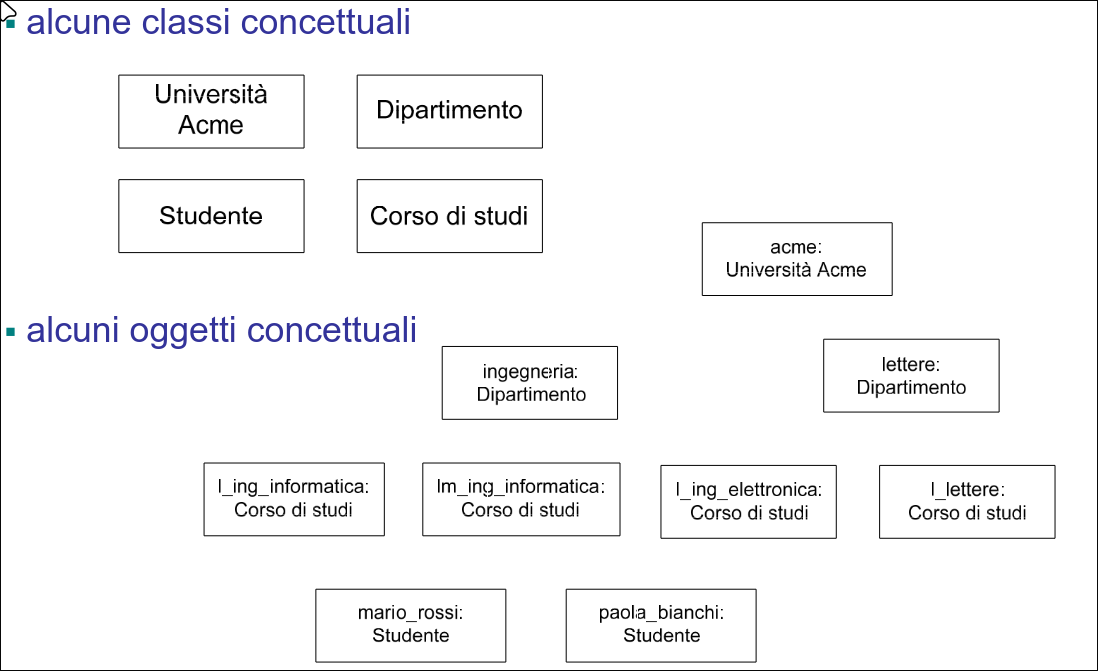
\includegraphics[width=\textwidth]{images/classi e oggetti concettuali.png}
\end{center}
\Large\textbf{Gli oggetti sono distinti dall'uso di :}\normalsize

\end{document}